\caulc
\begin{ex}%[1D1N3-1]
	Chọn phát biểu \textbf{đúng} trong các phát biểu sau.
	\choice
	{$\sin 2 x=\sin x \cos x$}
	{\True $\cos 2 x=\cos ^2 x-\sin ^2 x$}
	{$\tan x=\cot x$}
	{$\cot x \cdot \tan x=-1$}
	\loigiai{
		Phát biểu đúng $\cos 2x=\cos ^2x-\sin ^2x$.
	}
\end{ex}

\begin{ex}%[1D1H4-3]
	Cho đồ thị hàm số $y=\cos x$ trên đoạn $[-2\pi; 2 \pi]$. Khẳng định nào sau đây \textbf{đúng}?
	\begin{center}
%		\begin{tikzpicture}[scale=1, line cap=round, line join=round, font=\footnotesize,>=stealth]
%			\def\p{3.141593}
%			\draw plot[domain=-2*\p:2*\p, smooth](\x,{cos(\x)});
%		\end{tikzpicture}
		\begin{tikzpicture}[scale=1, line cap=round, line join=round, font=\footnotesize,>=stealth]
			\def\p{3.141593}
			\begin{axis}[
				domain=-2*\p:2*\p, % khoảng giá trị x
				samples=200, % số lượng mẫu vẽ
				axis lines=middle, % trục tọa độ
				xtick={-2*\p, -1.5*\p, -\p, -0.5*\p, 0, 0.5*\p, \p, 1.5*\p, 2*\p}, % vị trí các điểm đánh dấu trên trục x
				xticklabels={$-2\pi$, $-\tfrac{3\pi}{2}$, $-\pi$, $-\tfrac{\pi}{2}$, $0$, $\tfrac{\pi}{2}$, $\pi$, $\tfrac{3\pi}{2}$, $2\pi$}, % nhãn cho các điểm đánh dấu
				ytick={-1, 0, 1}, % vị trí các điểm đánh dấu trên trục y
				ymin=-1.5, ymax=1.5, % giới hạn giá trị y
				xlabel={$x$}, ylabel={$y$}, % nhãn cho trục x và y
				grid=both, % lưới dọc và ngang
				minor grid style={gray!25}, % kiểu lưới phụ
				major grid style={gray!50} % kiểu lưới chính
				]
				\addplot[color=blue, thick] {cos(deg(x))}; % vẽ đồ thị hàm cos(x)
			\end{axis}
		\end{tikzpicture}
	\end{center}
	\choice
	{Hàm số đã cho đồng biến khoảng $(0; 1)$}
	{Hàm số đã cho đồng biến trên $(-2 \pi; 2 \pi)$}
	{\True Hàm số đã cho đồng biến trên $(\pi; 2 \pi)$}
	{Hàm số đã cho đồng biến trên $(-2 \pi;-\pi)$}
	\loigiai{
		Hàm số đã cho đồng biến trên các khoảng $(-\pi; 0)$ và $(\pi; 2 \pi)$.
	}
\end{ex}

\begin{ex}%[1D1H2-3]
	Rút gọn biểu thức $A=\sin \left(x+14^\circ\right) \sin \left(x+74^\circ\right)+\sin \left(x-76^\circ\right) \sin \left(x-16^\circ\right)$ ta được
	\choice
	{$A=\dfrac{1}{2}$}
	{$1$}
	{$0$}
	{$\dfrac{1}{4}$}
	\loigiai{
		Ta có
		$$
		\begin{aligned}
			A & =\sin \left(14^\circ+x\right) \cos \left(16^\circ-x\right)+\sin \left(76^\circ-x\right) \sin \left(16^\circ-x\right) \\
			& =\sin \left(14^\circ+x\right) \cos \left(16^\circ-x\right)+\cos \left(14^\circ+x\right) \sin \left(16^\circ-x\right)\\
			&=\sin \left(14^\circ+16^\circ+x-x\right)
			=\sin 30^\circ=\dfrac{1}{2}\cdot
		\end{aligned}
		$$
	}
\end{ex}
\begin{ex}%[1D2N2-3]
	Cho cấp số cộng $\left(u_n\right)$ có $u_1=21, d=3$. Số hạng tổng quát của cấp số cộng $u_n$ là
	\choice
	{$7 \cdot 3^n$}
	{\True $3n+18$}
	{$21+3n$}
	{$21-3n$}
	\loigiai{
		Áp dụng công thức số hạng tổng quát, ta có $u_n=21+(n-1) \cdot 3=3n+18$.
	}
\end{ex}
\begin{ex}%[1D2H2-6]
	Cho cấp số cộng có $u_2+u_{22}=68$. Tổng của $23$ số hạng đầu tiên là
	\choice
	{$1496$}
	{\True $782$}
	{$1632$}
	{$1360$}
	\loigiai{
		Ta có
		$$\begin{aligned}
			S_{23}&=\dfrac{23\left(u_1+u_{23}\right)}{2}
			=\dfrac{23\left(u_1+u_1+22 d\right)}{2} \\
			&=\dfrac{23\left(u_1+d+u_1+21 d\right)}{2}
			=\dfrac{23\left(u_2+u_{22}\right)}{2}=\dfrac{23\cdot 68}{2}=782.
		\end{aligned}
		$$
	}
\end{ex}
\begin{ex}%[1D1N4-6]
	Tập giá trị của hàm số $y=\sin 3 x$ là
	\choice
	{$[0; 3]$}
	{\True $[-1; 1]$}
	{$[-3; 3]$}
	{$[-3; 1]$}
	\loigiai{
		$\forall x \in \mathbb{R}$, ta có $-1 \leq \sin 3 x \leq 1$ nên tập giá trị là $[-1; 1]$.
	}
\end{ex}
\begin{ex}%[1D1H5-5]
	Tập nào sau đây là tập nghiệm của phương trình $\sin 2 x+\cos 4 x=0$?
	\choice
	{\True $S=\left\{\dfrac{\pi}{4}+k\pi;-\dfrac{\pi}{12}+k \dfrac{\pi}{3}, k \in \mathbb{Z}\right\}$}
	{$S=\left\{\dfrac{\pi}{4}+k2 \pi;-\dfrac{\pi}{12}+k \dfrac{2 \pi}{3}, k \in \mathbb{Z}\right\}$}
	{$S=\left\{-\dfrac{\pi}{4}+k \pi; \dfrac{\pi}{12}+k \dfrac{\pi}{3}, k \in \mathbb{Z}\right\}$}
	{$S=\left\{-\dfrac{\pi}{4}+k 2 \pi; \dfrac{\pi}{12}+k \dfrac{2 \pi}{3}, k \in \mathbb{Z}\right\}$}
	\loigiai{
		Ta có
		$$
		\begin{aligned}
			& \sin 2x+\cos 4x=0 
			\Leftrightarrow \cos 4x=-\sin 2x 
			\Leftrightarrow \cos 4 x=\cos \left(\dfrac{\pi}{2}+2 x\right) \\
			& \Leftrightarrow \hoac{
				&4x = \dfrac{\pi}{2} + 2x + k2\pi \\
				&4 x = - \dfrac{\pi}{2} - 2x + k2\pi}
			\Leftrightarrow \hoac{&x=\dfrac{\pi}{4}+k\pi \\ &x=-\dfrac{\pi}{12}+k \dfrac{\pi}{3}}\,\, (k \in \mathbb{Z}).
		\end{aligned}
		$$
	}
\end{ex}
\begin{ex}%[1D2H2-4]
	Hàm số $u_n=7n-1$ xác đạnh trên tập hợp $M=\{1; 2; 3; 4; 5\}$ là một dãy số hữu hạn. Số hạng đầu và số hạng cuối của dãy số đó là
	\choice
	{\True $u_1=6, u_5=34$}
	{$u_1=7, u_5=35$}
	{$u_1=8, u_5=12$}
	{$u_1=1, u_5=5$}
	\loigiai{
		Ta có $u_1=7\cdot 1-1=6$; $u_5=7\cdot 5-1=34$.
	}
\end{ex}
\begin{ex}%[1D2H3-2]
	Trong các dãy số $\left(u_n\right)$ sau đây, dãy số nào là cấp số nhân?
	\choice
	{$u_n=3n$}
	{\True $u_n=2^n$}
	{$u_n=\dfrac{1}{n}$}
	{$u_n=2^n+1$}
	\loigiai{
		Xét dãy số $\left(u_n\right)$ với số hạng tổng quát $u_n=2^n$, ta có
		$$u_{n+1}=2^{n+1}=2\cdot 2^n=2u_n\,\, \forall n \in \mathbb{N}^*.$$
		Do đó dãy số $\left(u_n\right)$ là một cấp số nhân với công bội $q=2$.
	}
\end{ex}
\begin{ex}%[1D2H3-6]
	Cho cấp số nhân $\left(u_n\right)$ có $u_1=-3$ và $q=-2$. Tính tổng $10$ số hạng đầu tiên của cấp số nhân.
	\choice
	{$S_{10}=-511$}
	{$S_{10}=1023$}
	{$S_{10}=1025$}
	{$S_{10}=-1025$}
	\loigiai{
		Ta có $S_{10}=\dfrac{u_1\left(1-q^{10}\right)}{1-q}=\dfrac{-3\left(1-(-2)^{10}\right)}{1-(-2)}=1023$.
	}
\end{ex}
\begin{ex}%[1D3H2-3]
	Giới hạn $\lim\limits_{x\to +\infty} \dfrac{2x^5-3x^3+1}{4x^3-2x^4-x^5-3}$ bằng
	\choice
	{\True $-2$}
	{$\dfrac{1}{2}$}
	{$-3$}
	{$\dfrac{3}{2}$}
	\loigiai{
		Ta có $
		\lim\limits_{x\to +\infty} \dfrac{2x^5-3x^3+1}{4x^3-2x^4-x^5-3}
		=\lim\limits_{x\to +\infty} \dfrac{2-\dfrac{3}{x^2}+\dfrac{1}{x^5}}{\dfrac{4}{x^2}-\dfrac{2}{x}-1-\dfrac{3}{x^5}}
		=\dfrac{2}{-1}=-2$.
	}
\end{ex}
\begin{ex}%[1D3N2-2]
	Cho các giới hạn: $\lim\limits_{x\to  x_0} f(x)=2; \lim\limits_{x\to  x_0} g(x)=3$, hỏi $\lim\limits_{x\to  x_0}[3 f(x)-4 g(x)]$ bằng
	\choice
	{$5$}
	{$2$}
	{\True $-6$}
	{$3$}
	\loigiai{
		Ta có $\lim\limits_{x\to  x_0}\, \left[3f(x)-4g(x)\right]
		=3\lim\limits_{x\to  x_0} f(x)-4 \lim\limits_{x\to  x_0} g(x)
		=3\cdot 2-4\cdot 3=-6$.
	}
\end{ex}
\cauds
\begin{ex}%[1D1H4-6]
	Cho các hàm số $f(x)=\sqrt{3-2\sin x}$.
	\choiceTF
	{\True Hàm số $f(x)$ có tập xác định là $D=\mathbb{R}$}
	{\True Hàm số $f(x)$ đã cho là hàm tuần hoàn}
	{Hàm số $f(x)$ đã cho là hàm số chẵn}
	{Hàm số $f(x)$ có giá trị lớn nhất bằng $5$}
	\loigiai{
		\begin{itemchoice}
			\itemch Hàm số xác định khi: $3-2 \sin x \geq 0 \Leftrightarrow \sin x \leq \dfrac{3}{2}$. \\
				Vì vậy tập xác định hàm số là: $D=\mathbb{R}$.
			\itemch Với mọi $x \in \mathscr{D}$ thì $\heva{&x \pm 2\pi \in \mathscr{D} \\ 
				&&f(x+2 \pi)=\sqrt{3-2\sin (x+2\pi)}=\sqrt{3-2\sin x}=f(x).}$ \\
			Vậy hàm số đã cho là hàm tuần hoàn.
			\itemch Với mọi $x\in \mathscr{D}$, ta có 
			$\heva{&-x\in \mathscr{D} \\ &f(-x)=\sqrt{3-2 \sin (-x)}=\sqrt{3+2 \sin x} \neq f(x)}$, do đó hàm số $f(x)$ đã cho là không phải hàm số chẵn.
			\itemch Với mọi $x\in \mathscr{D}$, ta có $-1 \leq \sin x \leq 1; \forall x \in \mathbb{R} \Rightarrow 1 \leq 3-2 \sin x \leq 5 \Rightarrow 1 \leq \sqrt{3-2 \sin x} \leq \sqrt{5}$. Vậy hàm số $f(x)$ có giá trị lớn nhất bằng $\sqrt{5}$.
		\end{itemchoice}
	}
\end{ex}
\begin{ex}%[1D1H4-6]
	Cho hàm số $y=3-\sin \left(2x+\dfrac{\pi}{4}\right)$.
	\choiceTF
	{\True Hàm số có tập xác định $\mathscr{D}=\mathbb{R}$}
	{Giá trị lớn nhất của hàm số bằng $3$}
	{Tập giá trị của hàm số là $T=[1; 4]$}
	{\True Đồ thị hàm số không cắt trục hoành}
	\loigiai{
		\begin{itemchoice}
			\itemch Hàm số $y=3-\sin \left(2x+\dfrac{\pi}{4}\right)$ có tập xác định $\mathscr{D}=\mathbb{R}$.
			\itemch Dựa vào đường tròn lượng giác, với mọi $x$, ta có
			$$\begin{aligned}
				-1 \leq \sin \left(2x+\dfrac{\pi}{4}\right) \leq 1 
				\Leftrightarrow& 1 \geq-\sin \left(2 x+\dfrac{\pi}{4}\right) \geq-1 \\
				\Leftrightarrow& 4 \geq 3-\sin \left(2x+\dfrac{\pi}{4}\right) \geq 2 
				\Leftrightarrow 2\leq y \leq 4.
			\end{aligned}$$
			Vậy giá trị lớn nhất của hàm số bằng $4$.
			\itemch Và tập giá trị của hàm số là $T=[2; 4]$.
			\itemch Ta có $y\geq 2$ nên đồ thị hàm số đã cho không cắt trục hoành.
		\end{itemchoice}
	}
\end{ex}
\begin{ex}%[1D2H3-4]
	Cho cấp số nhân $\left(u_n\right)$ với công bội $q<0$ và $u_2=4, u_4=9$.
	\choiceTF
	{\True Số hạng đầu $u_1=-\dfrac{8}{3}$}
	{Số hạng $u_5=\dfrac{27}{2}$}
	{$-\dfrac{2187}{32}$ là số hạng thứ $8$}
	{\True Cấp số nhân có công bội $q=-\dfrac{3}{2}$}
	\loigiai{
		Ta có $u_2=u_1\cdot q=4, u_4=u_1\cdot q^3=9 
		\Rightarrow \dfrac{u_4}{u_2}=\dfrac{u_1 q^3}{u_1 q} 
		\Rightarrow \dfrac{9}{4}=q^2 
		\Rightarrow q=-\dfrac{3}{2}\,\, (q<0)$. \\
		Thay $q=-\dfrac{3}{2}$ vào $u_2$, ta được $u_1\left(-\dfrac{3}{2}\right)=4 \Rightarrow u_1=-\dfrac{8}{3}$. \\
		Số hạng tổng quát $u_n=-\dfrac{8}{3}\cdot \left(-\dfrac{3}{2}\right)^{n-1}$.
		\begin{itemchoice}
			\itemch Vậy cấp số nhân đã cho có số hạng đầu $u_1=-\dfrac{8}{3}$ và công bội $q=-\dfrac{3}{2}$.
			\itemch Khi đó $u_n=-\dfrac{8}{3} \cdot\left(-\dfrac{3}{2}\right)^{n-1} \Rightarrow u_5=-\dfrac{27}{2}\cdot$
			\itemch Ta có $-\dfrac{2187}{32} \neq -\dfrac{8}{3} \cdot\left(-\dfrac{3}{2}\right)^7$ nên không phải là số hạng thứ $8$.
			\itemch Cấp số nhân có công bội $q=-\dfrac{3}{2}\cdot$
		\end{itemchoice}
	}
\end{ex}

\begin{ex}%[1D3H2-7]
	Cho hàm số $f(x)=\heva{x-2 & \text { khi } x<-1 \\ \sqrt{x^2+1} & \text { khi } x \geq -1.}$
	\choiceTF
	{Giới hạn $\lim\limits_{x\to -2} f(x)=\sqrt{5}$}
	{\True Giới hạn $\lim\limits_{x\to -1^{-}} f(x)=-3$}
	{\True Giới hạn $\lim\limits_{x\to  -1^+}\, f(x)=\sqrt{2}$}
	{\True Hàm số tồn tại giới hạn khi $x \to -1$}
	\loigiai{
		\begin{itemchoice}
			\itemch Giới hạn $\lim\limits_{x\to -2} f(x)=-4$.
			\itemch Xét dãy số $\left(x_n\right)$ bất kì sao cho $x_n<-1$ và $x_n \to -1$, ta có: $f\left(x_n\right)=x_n-2$. \\
			Khi đó $\lim\limits_{x\to -1^-} f(x)=\lim f\left(x_n\right)=-1-2=-3$.
			\itemch Xét dãy số $\left(x_n\right)$ bất kì sao cho $x_n>-1$ và $x_n \rightarrow-1$, ta có: $f\left(x_n\right)=\sqrt{x_n^2+1}$.\\
			Khi đó $\lim\limits_{x\to -1^+} f(x)=\lim f\left(x_n\right)=\sqrt{(-1)^2+1}=\sqrt{2}$.
			\itemch Vì $\lim\limits_{x\to -1^{-}} f(x) \neq \lim\limits_{x\to -1^+} f(x)$ nên không tồn tại $\lim\limits_{x\to -1} f(x)$.
		\end{itemchoice}
	}
\end{ex}
\caukq
\begin{ex}%[1D1V5-3]
	Tìm số nghiệm thuộc đoạn $[0; 2025\pi]$ của phương trình $\sin \left(x+\dfrac{\pi}{4}\right)=0$.
	\shortans[0]{2025}
	\loigiai{
		Ta có $\sin \left(x+\dfrac{\pi}{4}\right)=0 \Leftrightarrow x+\dfrac{\pi}{4}=k \pi \Leftrightarrow x=-\dfrac{\pi}{4}+k \pi, k \in \mathbb{Z}$. \\
		Mà $x \in[0; 2025 \pi] \Rightarrow 0 \leq-\dfrac{\pi}{4}+k \pi \leq 2025 \pi \Leftrightarrow \dfrac{1}{4} \leq k \leq \dfrac{8101}{4}$. \\
		Do $k\in \mathbb{Z}$ nên $k \in\{1; 2; 3;\ldots; 2025\}$.
		Vậy phương trình có $2025$ nghiệm trên đoạn $[0; 2025 \pi]$.
	}
\end{ex}
\begin{ex}%[1D1C5-6]
	Giả sử một vật dao động điều hoà xung quanh vị trí cân bằng theo phương trình
	$$x=4 \cos \left(3 t+\dfrac{\pi}{6}\right).$$
	Ở đây, thời gian $t$ tính bằng giây và quãng đường $x$ tính bằng centimét. Hãy cho biết trong khoảng thời gian từ $0$ đến $16$ giây, vật đi qua vị trí cân bằng bao nhiêu lần?
	\shortans[]{15}
	\loigiai{
		Khi vật qua vị trí cân bằng, ta có $x=0$. Khi đó
		$$
		\begin{aligned}
			& 4 \cos \left(3 t+\dfrac{\pi}{6}\right)=0 \Leftrightarrow \cos \left(3 t+\dfrac{\pi}{6}\right)=0 \\
			& \Leftrightarrow 3 t+\dfrac{\pi}{6}=\dfrac{\pi}{2}+k \pi, k \in \mathbb{Z} \Leftrightarrow t=\dfrac{\pi}{9}+k \dfrac{\pi}{3}, k \in \mathbb{Z}.
		\end{aligned}
		$$
		Trong khoảng thời gian từ $0$ đến $16$ giây, tức là $0 \leq t \leq 16$ hay
		$$
		0 \leq \dfrac{\pi}{9}+k \dfrac{\pi}{3} \leq 16 \Leftrightarrow-\dfrac{1}{3} \leq k \leq \dfrac{48}{\pi}-\dfrac{1}{3}.
		$$
		Vì $k \in \mathbb{Z}$ nên $k \in\{0; 1, 2,\ldots, 14\}$. \\
		Vậy trong khoảng thời gian từ $0$ đến $16$ giây, vật đi qua vị trí cân bằng $15$ lần.
	}
\end{ex}
\begin{ex}%[1D2C2-7]
	An định xếp một hình tháp bởi các mảnh ghép tam giác. Tầng dưới cùng An xếp $35$ hình và tầng tiếp theo ít hơn tầng dưới nó hai hình. An xếp cho đến khi không xếp lên được nữa. Hỏi An cần bao nhiêu mảnh ghép hình tam giác để xếp xong tháp?
	\shortans[]{324}
	\begin{center}
%		\begin{tikzpicture}[scale=1, line join=round, line cap=round, font=\footnotesize,>=stealth]
%			\def\canh{4}
%			\path (0,0) coordinate (A)++(0:\canh) coordinate (B)++(120:\canh) coordinate (C);
%			\draw (A)--(B)--(C)--cycle;
%			\foreach \row in {1,2,3} {
%				\draw ($(A)!\row/4!(B)$)--++(120:\row);
%				\draw ($(A)!\row/4!(B)$)--++(60:4-\row);
%				\draw ($(A)!\row/4!(C)$)--++(0:4-\row);
%			}
%		\end{tikzpicture}
		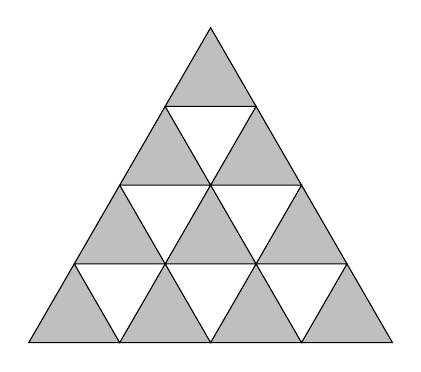
\begin{tikzpicture}
			\tikz\draw[fill=lightgray,even odd rule,xscale=2/sqrt(3),xslant=.5]
			(4,0)-|(0,4)--cycle (0,3)-|(1,0)--(0,1)-|(3,0)--cycle (0,2)-|(2,0)--cycle;
		\end{tikzpicture}
	\end{center}
	\loigiai{
		Theo giả thiết tòa tháp được xếp bằng các hình tam giác, số các tam giác xếp theo quy luật là một cấp số cộng. \\
		Gọi số tam giác tầng trên cùng là $u_1$ thì ta có $u_1=1, d=2$. \\
		Gọi tầng dưới cùng là $u_n \Rightarrow u_n=35$. \\
		Ta có $u_n=u_1+(n-1) d=35 \Leftrightarrow 1+(n-1) \cdot 2=35 \Leftrightarrow n=18 \Rightarrow S_{18}=\dfrac{18(1+35)}{2}=324$. \\
		Vậy tổng số tam giác trong $18$ tòa tháp trên là $S=324$.
	}
\end{ex}
\begin{ex}%[1D2C3-7]
	\immini{
		Cho hình vuông $ABCD$ có cạnh bằng $4$ và có diện tích $S_1$. Nối $4$ trung điểm $A_1, B_1, C_1, D_1$ theo thứ tự của $4$ cạnh $AB, BC, CD, DA$ ta được hình vuông thứ hai có diện tích $S_2$. Tiếp tục làm như thế, ta được hình vuông thứ ba là $A_2B_2C_2D_2$ có diện tích $S_3, \ldots$ và cứ tiếp tục làm như thế, ta tính được các hình vuông lần lượt có diện tích $S_4, S_5, \ldots, S_{100}$. Tính tổng $S=S_1+S_2+S_3+\ldots+S_{100}$.
		\shortans[]{32}
	}
	{
		\begin{tikzpicture}[scale=1, line join=round, line cap=round, font=\footnotesize,>=stealth]
			\pgfmathsetmacro\a{sqrt(2)} \def\canh{3}
			\path (0,0) coordinate (O);
			\foreach \i/\j in {0/A,1/B,2/C,3/D}{
				\path (45+90*\i:\canh) coordinate (\j);
			}
			\foreach \i/\j in {0/A1,1/B1,2/C1,3/D1}{
				\path (90+90*\i:\canh/\a) coordinate (\j);
			}
			\foreach \i/\j in {0/A2,1/B2,2/C2,3/D2}{
				\path (90+45+90*\i:\canh/2) coordinate (\j);
			}
			%\path (0,0) coordinate (A)++(0:\canh) coordinate (B)++(120:\canh) coordinate (C);
			\draw (A)--(B)--(C)--(D)--cycle
			(A1)--(B1)--(C1)--(D1)--cycle
			(A2)--(B2)--(C2)--(D2)--cycle;
			\foreach \a/\b in {A/45,B/135,C/270,D/-45,A1/90,B1/180,C1/-90,D1/0,A2/135,B2/-135,C2/-45,D2/45}{
				\fill[black] (\a)circle(.7pt) ($(\a)+(\b:2mm)$)node[scale=.8]{$\a$};
			}
		\end{tikzpicture}
	}
	\loigiai{
		Ta có $S_1=4^2; S_2=\dfrac{1}{2} 4^2=\dfrac{1}{2} S_1; S_3=\dfrac{1}{2} \cdot S_2=\dfrac{1}{2^2} \cdot S_1, \ldots$\\
		Suy ra $S=S_1+S_2+S_3+\ldots+S_{100}=S_1+\dfrac{1}{2} S_1+\dfrac{1}{2^2} S_1+\ldots+\dfrac{1}{2^{99}} S_1=S_1\left(1+\dfrac{1}{2}+\dfrac{1}{2^2}+\ldots+\dfrac{1}{2^{99}}\right)$
		Do đó $S_1, S_2, S_3, \ldots, S_{100}$ là cấp số nhân với số hạng đầu $u_1=S_1=4^2$ và công bội $q=\dfrac{1}{2}$.
		Vây $S=S_1 \cdot \dfrac{1-q^n}{1-q}=\dfrac{4^2\left(2^{100}-1\right)}{2^{99}}=32$.
	}
\end{ex}
\begin{ex}%[1D2C3-8]
	\immini{
		Cho hình vuông $ABCD$ có độ dài bằng $1$. Nối các trung điểm của bốn cạnh hình vuông $ABCD$, ta được hình vuông thứ hai. Tiếp tục nối các trung điểm của bốn cạnh hình vuông thứ hai, ta được hình vuông thứ ba. Tiếp tục như thế ta nhận được một dãy các hình vuông. Tìm tổng chu vi của dãy các hình vuông đó.
		\shortans[]{13,7}
	}
	{
		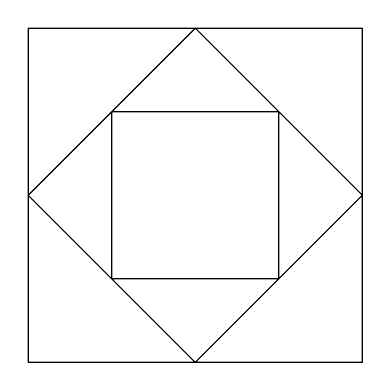
\begin{tikzpicture}[scale=1, line join=round, line cap=round, font=\footnotesize,>=stealth]
			\pgfmathsetmacro\a{sqrt(2)} \def\canh{3}
			\path (0,0) coordinate (O);
			\foreach \i/\j in {0/A,1/B,2/C,3/D}{
				\path (45+90*\i:\canh) coordinate (\j);
			}
			\foreach \i/\j in {0/A1,1/B1,2/C1,3/D1}{
				\path (90+90*\i:\canh/\a) coordinate (\j);
			}
			\foreach \i/\j in {0/A2,1/B2,2/C2,3/D2}{
				\path (90+45+90*\i:\canh/2) coordinate (\j);
			}
			%\path (0,0) coordinate (A)++(0:\canh) coordinate (B)++(120:\canh) coordinate (C);
			\draw (A)--(B)--(C)--(D)--cycle
			(A1)--(B1)--(C1)--(D1)--cycle
			(A2)--(B2)--(C2)--(D2)--cycle;
			%			\foreach \a/\b in {A/135,B/45,C/}{
				%				\draw ($(A)!\row/4!(B)$)--++(120:\row);
				%				\draw ($(A)!\row/4!(B)$)--++(60:4-\row);
				%				\draw ($(A)!\row/4!(C)$)--++(0:4-\row);
				%			}
		\end{tikzpicture}
	}
	\loigiai{
		Nếu cạnh hình vuông ban đầu là $x$ thì theo định lí Pythagore, ta có cạnh hình vuông thứ hai là $\sqrt{\left(\dfrac{x}{2}\right)^2+\left(\dfrac{x}{2}\right)^2}=\dfrac{x \sqrt{2}}{2}$\hfill $(*)$ \\
		Gọi cạnh hình vuông $ABCD$ là $u_1=1$, từ $(*)$ ta có cạnh hình vuông thứ hai là $u_2=\dfrac{\sqrt{2}}{2}$, cạnh hình vuông thứ ba là $u_3=\dfrac{1}{2}$, cạnh hình vuông thứ tư là $u_4=\dfrac{\sqrt{2}}{4}, \ldots$ \\
		Xét tổng chu vi dãy các hình vuông là
		$S=4u_1+4u_2+4 u_3+\ldots =4\left(1+\dfrac{\sqrt{2}}{2}+\dfrac{1}{2}+\dfrac{\sqrt{2}}{4}+\ldots\right)$. \\
		Dễ thấy $1+\dfrac{\sqrt{2}}{2}+\dfrac{1}{2}+\dfrac{\sqrt{2}}{4}+\ldots$ là tổng của cấp số nhân lùi vô hạn có số hạng đầu bằng $1$, công bội bằng $\dfrac{\sqrt{2}}{2}$. \\
		Vậy ta có $S=4 \cdot \dfrac{u_1}{1-q}=4 \cdot \dfrac{1}{1-\dfrac{\sqrt{2}}{2}}=8+4 \sqrt{2}=13{,}7$.
	}
\end{ex}
\begin{ex}%[1D3V2-8]
	Chi phí để sản xuất $x$ sản phẩm của một công ty được xác định bởi hàm số: $C(x)=50000+105 x$. Khi số sån phẩm sản xuất ra ngày càng nhiều thì chi phí trung bình chỉ tối đa là bao nhiêu nghìn đồng?
	\shortans[]{105}
	\loigiai{
		Chi phí trung bình $\overline{C}(x)$ để sản xuất một sản phẩm là $\overline{C}(x)=\dfrac{50000+105x}{x}$. \\
		Ta có 
		$$\begin{aligned}
			\lim\limits_{x\to +\infty} \overline{C}(x)
			&=\lim\limits_{x\to +\infty} \dfrac{50000+105 x}{x}
			=\lim\limits_{x\to +\infty} \dfrac{x\left(\dfrac{50000}{x}+105\right)}{x} \\
			&=\lim\limits_{x\to +\infty}\left(\dfrac{50000}{x}+105\right)=105.
		\end{aligned}$$
		Khi số sản phẩm sản xuất ra ngày càng nhiều thì chi phí trung bình chỉ tối đa là $105$ nghìn.
	}
\end{ex}